\section{Исследовательская часть}

В данном разделе проверяется успешности чтения сертификата участниками сети. Приводится исследование времени финализации транзакций в сети с разным количеством узлов. Также выполнено cравнение реализованного метода с аналогами.


\subsection{Проверка успешности чтения сертификата}

Созданный сертификат принадлежит выпускнику и учебному заведению, что его выдало. Соответственно, прочитать этот сертификат могут только эти два участника сети. Чтобы подтвердить это утверждение был проведен соответствующий эксперимент.

Для проведения эксперимента потребовались следующие входные данные:
\begin{itemize}[leftmargin=1.6\parindent]
	\item[---] адрес $addr$ смарт"=контракта некоторой тестовой учебной организации (0x0x9f7F6a7C28e9d0733fD2d59071bA500B54430044);
	\item[---] публичный ключ $A$ выпускника №1 \\
	(0x6Be02d1d3665660d22FF9624b7BE0551ee1Ac91b);
	\item[---] публичный ключ $B$ выпускника №2 \\
	(0x8097c3C354652CB1EEed3E5B65fBa2576470678A).
\end{itemize}

В рамках эксперимента был создан смарт"=контракт некоторой тестовой учебной организации под адресом $addr$. Далее был создан сертификат, выданный участнику $A$ (рисунок \ref{fig:a10}). Далее участник $A$ успешно <<прочитал>> выданный ему сертификат (скриншот прочтения сертификата изображен на рисунке \ref{fig:a11}). При попытке прочитать тот же самый сертификат участником $B$, вместо метаданных сертификата пользователь получил информацию об ошибке чтения, которая приведена на рисунке \ref{fig:a12}.

\begin{figure}[h!]
	\centering
	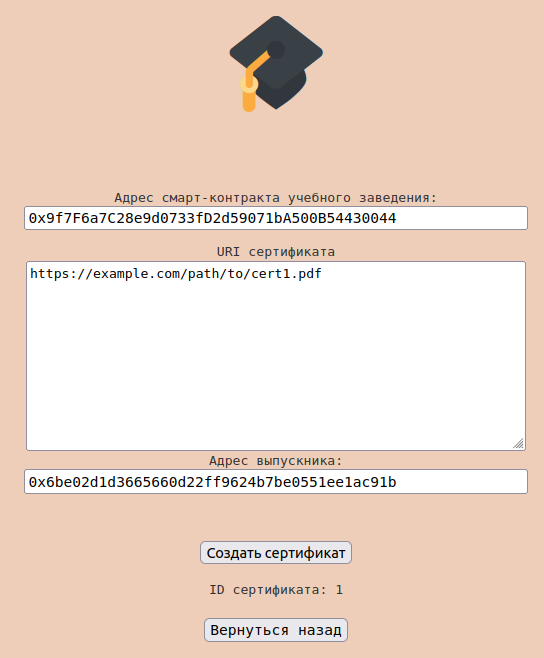
\includegraphics[width=\textwidth]{img/cert_created.png}
	\caption{Создание уникального сертификата}
	\label{fig:a10}
\end{figure}

\begin{figure}[h!]
	\centering
	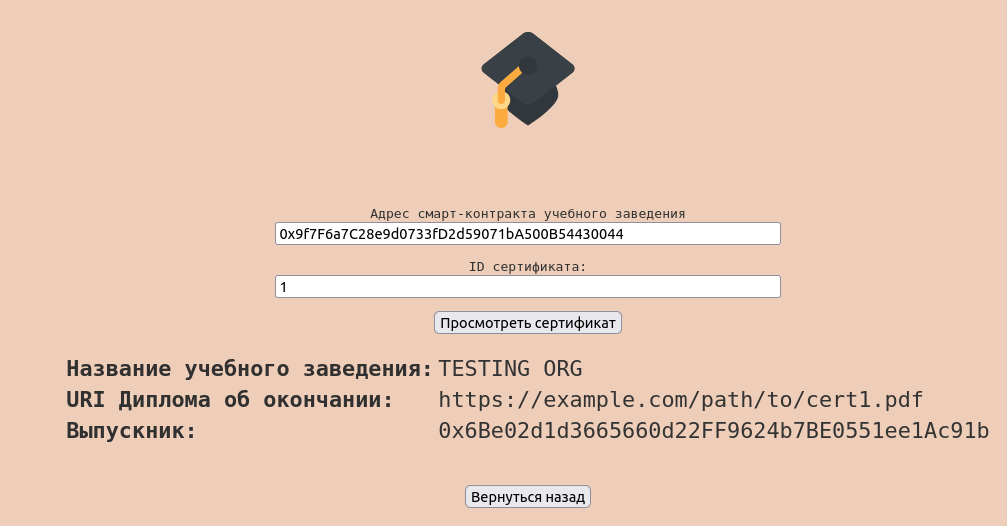
\includegraphics[width=\textwidth]{img/cert_seen.png}
	\caption{Чтение сертификата выпускником-владельцем этого сертификата}
	\label{fig:a11}
\end{figure}

\begin{figure}[h!]
	\centering
	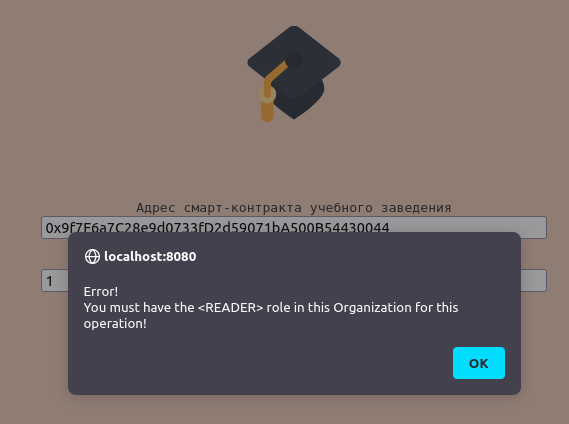
\includegraphics[width=\textwidth]{img/cert_not_seen.png}
	\caption{Чтение сертификата другим участником сети}
	\label{fig:a12}
\end{figure}

Проведя данный эксперимент, было получено подтверждение утверждения о том, что только владелец сертификата может его прочитать. Таким образом, можно судить о конфиденциальности сертификатов в сети: злоумышленики не будут иметь доступ к сертификатам, а соответственно и документам, других пользователей.

\subsection{Проведение исследования времени финализации транзакций в сети}

Было проведено исследование зависимости времени финализации транзакций, от количества участников"=валидаторов в сети. Для этого были произведены замеры времени финализации транзакций в сети с 1, 2, 3, 4 и 5 валидаторами.

В качестве замеряемых транзакций были выбраны транзакции создания смарт"=контракта учебного заведения и выдачи уникального сертификата выпускнику. Для каждого количества участников сети и было произведено по 5 замеров времени финализации каждой транзакции и взято соответствующее среднее значение. На рисунках \ref{fig:a13} и \ref{fig:a14} приведены столбиковые диаграммы результатов замеров времени финализации транзакции создания смарт"=контракта учебного заведения и выдачи сертификата выпускнику, соответственно.


\begin{figure}[!htb]
	\centering
	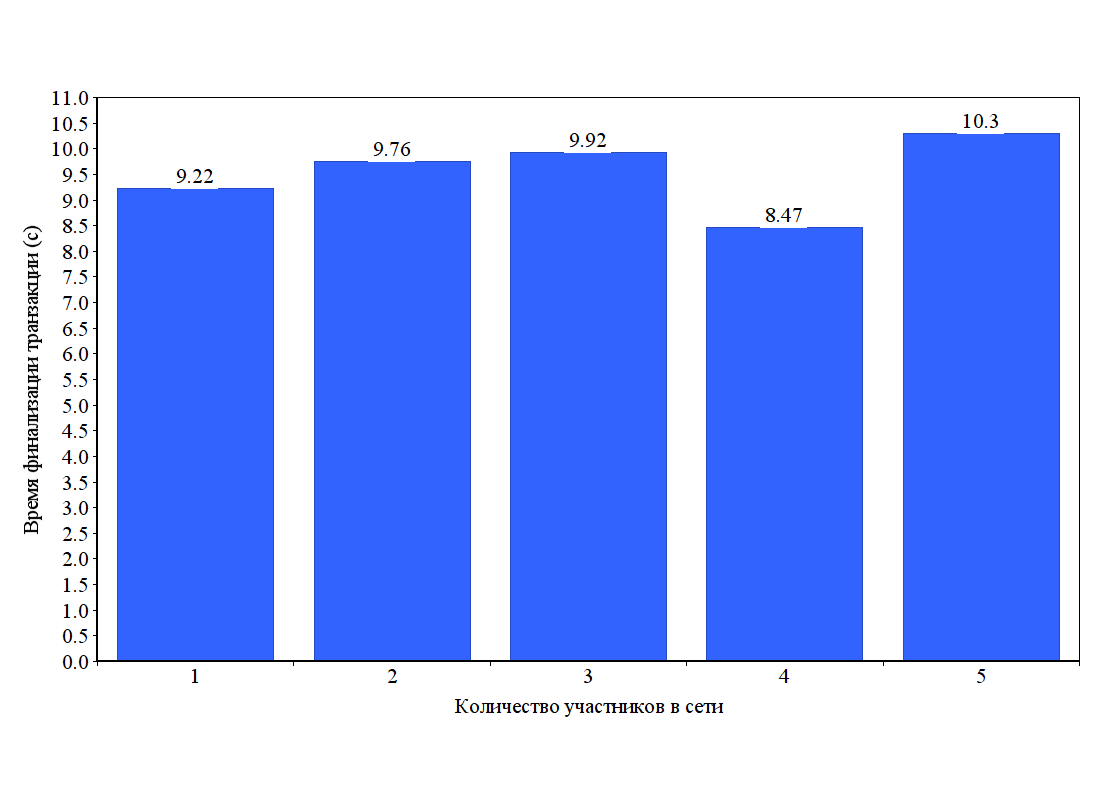
\includegraphics[width=\textwidth - 40pt]{img/t_org.png}
	\caption{Зависимость времени финализации транзакции создания смарт-контракта учебного заведения от количества участников в сети}
	\label{fig:a13}
\end{figure}


\begin{figure}[!htb]
	\centering
	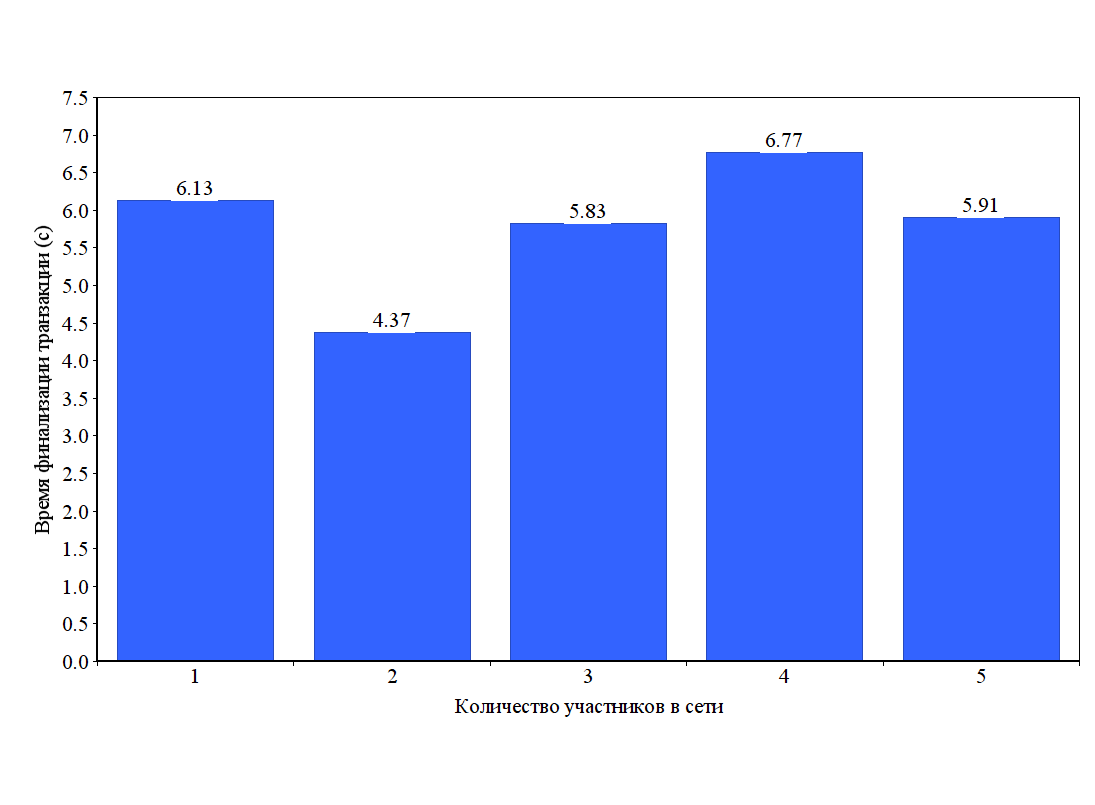
\includegraphics[width=\textwidth - 40pt]{img/t_token.png}
	\caption{Зависимость времени финализации транзакции создания уникального сертификата от количества участников в сети}
	\label{fig:a14}
\end{figure}

Дисперсии полученных результатов зависимости времени финализации транзакции создания смарт-контракта учебного заведения и создания уникального сертификата от количества участников в сети составляют $0.5044$ и $0.7769$ соответственно. Данные значения дисперсии говорят о кучности полученных значений -- полученные результаты релевантны.

На основании полученных результатов, можно сделать вывод, что время финализации транзакции как создания смарт"=контракта учебного заведения, так и создания уникального сертификата не зависит от количества участников в сети, а зависит от временных интервалов производства новых блоков и их финализации, а также времени распространения информации о новом блоком среди валидаторов сети. Данный вывод позволяет судить о том, что в будущем разработанную сеть можно будет успешно масштабировать на большее число участников.

Также отметим, что среднее время создания смарт"=контракта учебного заведения на 63\% больше, чем время создания уникального сертификата. Это обусловлено тем, что для создания смарт"=контракта виртуальная машина выполняет больше действий, нежели чем при создании невзаимозаменяемого токена.



\subsection{Сравнение реализованного метода с аналогами}

Было произведено сравнение разработанного метода с рассмотренными в аналитической части аналогами: сертификатами, выдаваемые образовательными онлайн-платформами, (Coursera, в частности), и документами об окончания вуза РФ.

Документы об окончания вуза РФ подвержены износу, их можно потерять. Чтобы их восстановить необходимо обращаться в уполномоченные органы. В то же время, предложенный метод персистентно хранит все сертификаты в блокчейне, лишая выпускника задач сохранения и восстановления выданных ему документов.

Сертификаты Coursera можно подделать (отредактировать) в текстовом редакторе. Предложенный же метод не подразумевает изменение созданных сертификатов, то есть однажды созданный сертификат больше нельзя отредактировать.

Чтобы проверить подлинность и сертификатов Coursera, и документов об окончании вуза РФ, необходимо сформировать официальный запрос и дождаться ответа на него. В свою очередь, реализованный метод позволяет получить подтверждение подлинности документов, не оформляя никаких запросов в уполномоченные организации, что существенно ускоряет время подтверждения.


На таблице 5 представлено сравнение реализованного метода с существующими реализациями выдачи сертификатов, подтверждающих окончание учебного заведения.
\begin{table}[h!]
	\captionsetup{justification=raggedleft,singlelinecheck=off}
	\caption{Сравнение реализованного метода с аналогами}
	\resizebox{\columnwidth}{!}{\begin{tabular}{| c | c | c | c | c |}
			\hline
			\backslashbox{Реализация}{Критерий} & Утрата & Износ & Подделывание & Проверка подлинности \\
			\hline
			Документы об окончания вуза РФ & - & - & + & - \\
			\hline
			Сертификаты Coursera & + & + & - & - \\
			\hline
			Предложенный метод & + & + & + & + \\
			\hline
	\end{tabular}}
\end{table}


\subsection*{Выводы}
\addcontentsline{toc}{subsection}{Выводы}

В данном раздела были проведены исследования успешности чтения сертификата участниками сети, а также зависимости времени финализации транзакций в сети с разным количеством узлов. В ходе данных исследований было установлено, что:
\begin{itemize}[leftmargin=1.6\parindent]
	\item[---] разработанные сертификаты конфиденциальны: личные данные в сертификате доступны только владельцу сертификата;
	\item[---] время финализации транзакции не зависит от количества участников в сети, а зависит от временных интервалов производства новых блоков и их финализации, а также времени распространения информации о новом блоком среди валидаторов сети;
	\item[---] среднее время создания смарт"=контракта учебного заведения примерно в полтора раза больше, чем время создания уникального сертификата.
\end{itemize} 

Также было произведено сравнение существующими аналогами выдачи сертификатов, подтверждающих окончание учебного заведения. Было установлено, что предложенный метод является предпочтительным.


\pagebreak